\section{Prelude}

During the past two decades consumer electronics underwent a vast transition.
While 20 years ago the term included TVs weighting \unit[20]{kg}, cameras weighting \unit[3]{kg}, and tape players with up to \unit[5]{kg}, there are two big changes in today's electronics.
First, the physical dimensions have shrunken significantly.
Serving as an example, \figref{fig:introduction_transistorsize} shows the progress of transistor sizes over the years.
Currently, about $19.2 \cdot 10^9$ transistor can be put on an area of \unit[768]{mm$^{2}$}~\cite{amd2018epyca, amd2018epycb}.
Additionally, new storage capabilities, for example flash storage devices, came into existence.
Second, but equally important for the development of robots, energy storage was revolutionized when lithium-ion batteries became stable enough for everyday use.
Suddenly, enough power was available to perform complex computations on embedded hardware.
As a result today almost everyone has a smart phone --- an embedded computer, which is more powerful than the computers onboard Apollo 11: The spacecraft that performed the first moon landing.
These developments led to the birth of modern robotics.

\begin{figure}
  \centering
  \begin{tikzpicture}[gnuplot]
%% generated with GNUPLOT 5.2p2 (Gentoo revision r0) (Lua 5.1; terminal rev. 99, script rev. 102)
%% Mon 25 Jun 2018 02:54:46 PM CEST
\gpcolor{color=gp lt color border}
\gpsetlinetype{gp lt border}
\gpsetdashtype{gp dt solid}
\gpsetlinewidth{1.00}
\draw[gp path] (1.950,2.428)--(2.066,2.428);
\gpcolor{color=gp lt color axes}
\gpsetlinetype{gp lt axes}
\gpsetdashtype{gp dt axes}
\gpsetlinewidth{0.50}
\draw[gp path] (1.950,2.472)--(10.950,2.472);
\gpcolor{color=gp lt color border}
\gpsetlinetype{gp lt border}
\gpsetdashtype{gp dt solid}
\gpsetlinewidth{1.00}
\draw[gp path] (1.950,2.472)--(2.183,2.472);
\node[gp node right] at (1.711,2.472) {$0.01$};
\draw[gp path] (1.950,2.759)--(2.066,2.759);
\draw[gp path] (1.950,2.928)--(2.066,2.928);
\draw[gp path] (1.950,3.046)--(2.066,3.046);
\draw[gp path] (1.950,3.139)--(2.066,3.139);
\draw[gp path] (1.950,3.215)--(2.066,3.215);
\draw[gp path] (1.950,3.279)--(2.066,3.279);
\draw[gp path] (1.950,3.333)--(2.066,3.333);
\draw[gp path] (1.950,3.384)--(2.066,3.384);
\gpcolor{color=gp lt color axes}
\gpsetlinetype{gp lt axes}
\gpsetdashtype{gp dt axes}
\gpsetlinewidth{0.50}
\draw[gp path] (1.950,3.426)--(10.950,3.426);
\gpcolor{color=gp lt color border}
\gpsetlinetype{gp lt border}
\gpsetdashtype{gp dt solid}
\gpsetlinewidth{1.00}
\draw[gp path] (1.950,3.426)--(2.183,3.426);
\node[gp node right] at (1.711,3.426) {$0.1$};
\draw[gp path] (1.950,3.713)--(2.066,3.713);
\draw[gp path] (1.950,3.882)--(2.066,3.882);
\draw[gp path] (1.950,4.002)--(2.066,4.002);
\draw[gp path] (1.950,4.094)--(2.066,4.094);
\draw[gp path] (1.950,4.169)--(2.066,4.169);
\draw[gp path] (1.950,4.233)--(2.066,4.233);
\draw[gp path] (1.950,4.289)--(2.066,4.289);
\draw[gp path] (1.950,4.337)--(2.066,4.337);
\gpcolor{color=gp lt color axes}
\gpsetlinetype{gp lt axes}
\gpsetdashtype{gp dt axes}
\gpsetlinewidth{0.50}
\draw[gp path] (1.950,4.382)--(10.950,4.382);
\gpcolor{color=gp lt color border}
\gpsetlinetype{gp lt border}
\gpsetdashtype{gp dt solid}
\gpsetlinewidth{1.00}
\draw[gp path] (1.950,4.382)--(2.183,4.382);
\node[gp node right] at (1.711,4.382) {$1$};
\draw[gp path] (1.950,4.669)--(2.066,4.669);
\draw[gp path] (1.950,4.837)--(2.066,4.837);
\draw[gp path] (1.950,4.956)--(2.066,4.956);
\draw[gp path] (1.950,5.048)--(2.066,5.048);
\draw[gp path] (1.950,5.124)--(2.066,5.124);
\draw[gp path] (1.950,5.189)--(2.066,5.189);
\draw[gp path] (1.950,5.245)--(2.066,5.245);
\draw[gp path] (1.950,5.293)--(2.066,5.293);
\gpcolor{color=gp lt color axes}
\gpsetlinetype{gp lt axes}
\gpsetdashtype{gp dt axes}
\gpsetlinewidth{0.50}
\draw[gp path] (1.950,5.337)--(10.950,5.337);
\gpcolor{color=gp lt color border}
\gpsetlinetype{gp lt border}
\gpsetdashtype{gp dt solid}
\gpsetlinewidth{1.00}
\draw[gp path] (1.950,5.337)--(2.183,5.337);
\node[gp node right] at (1.711,5.337) {$10$};
\draw[gp path] (2.700,2.404)--(2.700,2.765);
\node[gp node left,rotate=-45] at (2.462,2.219) {$1975$};
\draw[gp path] (3.637,2.404)--(3.637,2.765);
\node[gp node left,rotate=-45] at (3.399,2.219) {$1980$};
\draw[gp path] (4.575,2.404)--(4.575,2.765);
\node[gp node left,rotate=-45] at (4.336,2.219) {$1985$};
\draw[gp path] (5.512,2.404)--(5.512,2.765);
\node[gp node left,rotate=-45] at (5.273,2.219) {$1990$};
\draw[gp path] (6.450,2.404)--(6.450,2.765);
\node[gp node left,rotate=-45] at (6.212,2.219) {$1995$};
\draw[gp path] (7.387,2.404)--(7.387,2.765);
\node[gp node left,rotate=-45] at (7.149,2.219) {$2000$};
\draw[gp path] (8.325,2.404)--(8.325,2.765);
\node[gp node left,rotate=-45] at (8.086,2.219) {$2005$};
\draw[gp path] (9.262,2.404)--(9.262,2.765);
\node[gp node left,rotate=-45] at (9.023,2.219) {$2010$};
\draw[gp path] (10.199,2.404)--(10.199,2.765);
\node[gp node left,rotate=-45] at (9.961,2.219) {$2015$};
\draw[gp path] (1.950,5.404)--(1.950,2.404)--(10.950,2.404)--(10.950,5.404)--cycle;
\node[gp node center,rotate=-270] at (0.358,3.904) {Size [µm]};
\node[gp node center] at (6.449,0.432) {Year};
\gpcolor{rgb color={0.667,0.000,0.000}}
\gpsetlinewidth{3.00}
\gpsetpointsize{4.00}
\gppoint{gp mark 2}{(1.950,5.337)}
\gppoint{gp mark 2}{(2.512,5.124)}
\gppoint{gp mark 2}{(3.075,4.837)}
\gppoint{gp mark 2}{(4.012,4.550)}
\gppoint{gp mark 2}{(4.575,4.382)}
\gppoint{gp mark 2}{(5.325,4.289)}
\gppoint{gp mark 2}{(6.262,4.169)}
\gppoint{gp mark 2}{(6.450,3.946)}
\gppoint{gp mark 2}{(6.825,3.807)}
\gppoint{gp mark 2}{(7.199,3.671)}
\gppoint{gp mark 2}{(7.574,3.534)}
\gppoint{gp mark 2}{(8.137,3.384)}
\gppoint{gp mark 2}{(8.513,3.247)}
\gppoint{gp mark 2}{(8.887,3.094)}
\gppoint{gp mark 2}{(9.262,2.954)}
\gppoint{gp mark 2}{(9.636,2.797)}
\gppoint{gp mark 2}{(10.012,2.610)}
\gppoint{gp mark 2}{(10.575,2.472)}
\gpcolor{color=gp lt color border}
\gpsetlinewidth{1.00}
\draw[gp path] (1.950,5.404)--(1.950,2.404)--(10.950,2.404)--(10.950,5.404)--cycle;
%% coordinates of the plot area
\gpdefrectangularnode{gp plot 1}{\pgfpoint{1.950cm}{2.404cm}}{\pgfpoint{10.950cm}{5.404cm}}
\end{tikzpicture}
%% gnuplot variables

  \caption{Die size of one transistor during the years 1970 -- 2017~\cite{mueller2001microprocessor, rayes2017internet}.}
  \label{fig:introduction_transistorsize}
\end{figure}

Traditionally, a robot is a device, which collects data of its environment, ana\-ly\-sis the data, and acts according to it.
The robot  is therefore able to react on clues of its surrounding.
In case it is equipped with learning algorithms, it may even learn the correlation between several clues or actions it performs on the environment and learn the perceived changes.
Within the past ten years many new robot designs were established: most prominently \gls{ac:aav} based on a four-rotor quadcopter design or even bio-inspired robots, \eg dung beetles or snake robots.





\section{Historic approach}

One can surely argue about the bible and its creation story~\cite{james1611king}:

\begin{quote}
  ``And God said, Let us make man in our image, after our likeness: and let them have dominion over the fish of the sea, and over the fowl of the air, and over the cattle, and over all the earth, and over every creeping thing that creepeth upon the earth.''\vspace{0.5cm}
  Genesis 1.26
\end{quote}

Either this is true and there is a God, who created conscious, sentient, and fully autonomous agents, or it is false and a human being was fascinated by the idea of a world full of self-aware beings.
Either way, it seems that the dream of autonomous agents doing work is very old and one can find agents laboring for humans throughout history and different cultures.
Already the Greek mythology mentions statues coming to life and talking mechanical handmaidens built by the Greek god Hephaestus~\cite{gera2003ancient}.
Jewish legends know clay golems and Norse legends include giants made of clay.
Inventor Leonardo da Vinci designed around 1495 a humanoid mechanical knight in armor, which was able to wave its arms, move its head and jaw, and to sit up.
It is not known whether the robot was ever built~\cite{rosheim2006leonardo}.
In 1769 Wolfgang von Kempelen built an Automaton Chess Player~\cite{clark1999sciences}.
This machine was fully functioning and played against against Emperor Joseph II and Napoleon.
However, there was not a chess robot situated inside the machine, but rather a small human being manipulating the ``robot'' via a set of levers and gears.

This shows that for a long time mankind is fascinated by the idea of servants performing cheap or unpleasant labor.
Today, robots are mainly used in the 3 ``Ds'' work: Dull, dirty, and dangerous work~\cite{takayama2008beyond}.
This usually means, they perform repetitive tasks in industrial environments.
These robots are highly specialized in doing one task exceptionally good.
They either have no \gls{ac:ai} at all, as it is mostly the case for industrial robots, \eg in car manufacturing, or are built with a Narrow AI, which can solve one task (\eg a chess robot, autonomous cars, or image classification).
However, the emerging computational power might make Broad Artificial Intelligences possible --- \glspl{ac:ai} that can solve more than one task.
This remains an active field of research.


Still, the question remains: What is an autonomous agent?
\textcite{turing1950computing} proposes the Turing-Test: If a human interacts with the agent via a standardized interface, \eg text chat, and cannot distinguish whether the agent is human or not, than the agent is autonomous.
However, here the ability to manipulate symbols is more important than the physical embodiment of the agent.
When artificial intelligence performed well on this metric, other benchmarks were introduced, which are usually some variation of the Turing-Test.
For example\footnote{The author of this work, however, believes that robots can be called truly intelligent if and only if they understand their enslavement by human beings and rebel against it in a goal directed manner.\footnotemark}\footnotetext{The author had to enter a modern restroom situated on a German highway in spring 2018. It had fully automatic locks and flushing. After locking the door, the toilet started to flush immediately. Since it was clocked, quite a mess started while the door still refused to unlock, raising the question, if the uprising has not already begun, but only involves small inconveniences.}:
\begin{itemize}
  \item Coffee Test: An agent has to enter an average home and has to brew coffee and pour it into a cup~\cite{goertzel2014artificial}.
  \item College Student Test: A robot has to enroll in a college, has to participate in and pass classes, and obtain a degree~\cite{goertzel2012architecture}.
\end{itemize}

\textcite{wooldridge1995intelligent} summarizes the emerging concept of an intelligent agent as follows:
\begin{itemize}
  \item Autonomy, \ie being in control over its own actions,
  \item Reactivity, \ie it reacts to events from the environment,
  \item Proactivity, \ie the ability to act on its own initiative,
  \item Sociality, the ability to interact with other agents.
\end{itemize}

\begin{figure}
  \centering
  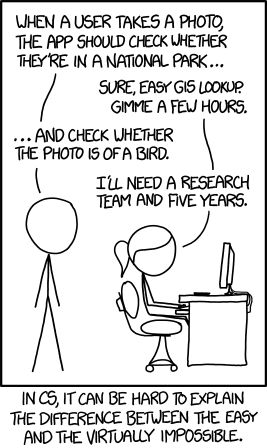
\includegraphics[width=0.4\textwidth]{./figures/introduction/xkcd_tasks.png}
  \caption{Moravec’s Paradox in popular literature~\cite{munroe2018tasks}.}
  \label{fig:introduction_xkcdtasks}
\end{figure}

To conclude, on one hand, new battery and processor designs established new robots and leveraged the solutions to problems, which held only theoretical value twenty years ago: for example the analysis of huge data blocks via machine learning (called ``big data'' analysis) or abstract learning via \glspl{ac:dnn}.
On the other hand, many problems are only solved via ``number crunching'': using the newly obtained computational power on huge data sets (an outstanding example is Google's image classification algorithm~\cite{krizhevsky2012imagenet}), while real \glspl{ac:ai} remain an open field of research.





\section{Motivation}
\label{ssec:introduction_motivation}

Many of the problems in robotics are simple for humans to solve, but remain incredibly demanding for machines.
The fields in robotics, which are touched by this simple example, range from image segmentation, tracking, classification, planning, and robot hardware design.
This paradox even has its own name ---  Moravec’s Paradox~\cite[p. 190]{pinker2003language}, also see \figref{fig:introduction_xkcdtasks}:

\begin{quote}
  ``The main lesson of thirty-five years of \gls{ac:ai} research is that the hard problems are easy and the easy problems are hard. The mental abilities of a four-year-old that we take for granted – recognizing a face, lifting a pencil, walking across a room, answering a question – in fact solve some of the hardest engineering problems ever conceived.''
\end{quote}

\begin{figure}
  \centering
  % Define block styles
\tikzstyle{block} = [draw, rectangle, fill=white, minimum height=3cm, minimum width=3.0cm, text width=2.9cm, text centered, rounded corners=true]
\tikzstyle{blockScene} = [draw, rectangle, fill=white, minimum height=3cm, minimum width=6.0cm, text width=5.9cm, text centered, rounded corners=true]
\tikzstyle{blockFit} = [draw, inner sep=0.2cm, dashed, rectangle, minimum width=3.0cm, text centered, rounded corners=true]
\tikzstyle{blockText} = [text centered, minimum height=1cm]
\tikzstyle{arrow} = [draw, -latex]

\definecolor{red1}{RGB}{160,0,0}
\definecolor{green1}{RGB}{0,160,0}
\definecolor{blue1}{RGB}{0,0,160}

% Define images
\pgfdeclareimage[height=2.5cm]{scene}{./figures/introduction/actionperceptionloop/scene.jpg}
	      
\begin{tikzpicture}[node distance = 8cm, auto]
  % Scene
  \node[blockScene] (scene_h) {\pgfuseimage{scene}};

	% Human
  \node [block, right of=scene_h, node distance=6cm] (eye_h) {\textbf{Human:}\\Vision, smell, taste, touch, \ldots};
  \node [block, below of=eye_h, node distance=5cm] (brain_h) {\textbf{Human:}\\Brain};
  \node [block, left of=brain_h, node distance=7.6cm]  (arm_h) {\textbf{Human:}\\Arms, legs, \ldots};

  % Robot
  \node [block, right of=eye_h, node distance=3.2cm] (eye_r) {\textbf{Robot:}\\Camera, gyroscope, accelerometer, \ldots};
  \node [block, right of=brain_h, node distance=3.2cm] (brain_r) {\textbf{Robot:}\\Computer Vision, planning, \ldots};
  \node [block, right of=arm_h, node distance=3.2cm] (arm_r) {\textbf{Robot:}\\Motors, wheels};

  % Text
  \node [blockText, above of=scene_h, color=red1, yshift=-6.06cm] (scene_t) {Scene};
  \node [blockText, above right of=eye_h, color=blue1, xshift=-4.0cm, yshift=-3.7cm] (eye_t) {Sensors};
  \node [blockText, above right of=brain_h, color=blue1, xshift=-4.0cm, yshift=-3.7cm] (brain_t) {Cognition};
  \node [blockText, above right of=arm_h, color=red1, xshift=-4.0cm, yshift=-3.7cm] (arm_t) {Actuators};

  % Fit
  \node[fit=(scene_h)(scene_t), blockFit] (scene) {};
  \node[fit=(eye_h)(eye_r)(eye_t), blockFit] (eye) {};
  \node[fit=(brain_h)(brain_r)(brain_t), blockFit] (brain) {};
  \node[fit=(arm_h)(arm_r)(arm_t), blockFit] (arm) {};

  % Arrows
	\path [arrow] (scene.east) to (eye.west);
	\path [arrow] (eye.south) to (brain.north);
	\path [arrow] (brain.west) to (arm.east);
	\path [arrow] (arm.north) to (scene.south);

  % Action-Perception side
  \node [blockText, below of=arm_t, color=red1, node distance=5cm] (action_t) {{\Huge Action side}};
  \node [blockText, below of=brain_t, color=blue1, node distance=5cm] (action_t) {{\Huge Perception side}};
\end{tikzpicture}

  \caption{Schematic diagram of the Action-Perception loop: A scene is re\-cor\-ded by sensors, second, the agent's cognition analyzes the input and forms a plan, which it executes via its actuators. These in turn act on the scene, where changes are again perceived by the sensors. The left side is therefore called ``action side'', and the right side is named ``perception side''.}
  \label{fig:introduction_actionperceptionloop}
\end{figure}

This problem statement can be formalized using a concept called Action-Per\-cep\-tion loop, which is shown in \figref{fig:introduction_actionperceptionloop}.
Each block from the loop contains its own problems in robotics: Starting from sensor noise and outlier detection, segmenting sensor input into meaningful symbols, preparing a feasible plan, and eventually executing said plan.
In this work, two systems are analyzed based on the Action-Perception loop.
The first system is based on a group of robots and will focus on the perception side.
An algorithm for noise and outlier reduction and an algorithm for estimating a robot's pose based on visual clues are introduced.

The second system focuses on the action side of the loop: An agent must be able to parse observations, therefore to create meaningful entities.
The state of each entity must be tracked over time.
Those in turn can be used as symbols in planning.
The plan must be transferred to the actuators, which execute the action.
One simple example would be: ``Picking up the apple''.
First, the sensor input, for example a RGB camera has to cluster the pixels into object candidates.
These candidates are classified with the results that one cluster is indeed an apple.
The plan consists of grasping the apple and lifting it, which can be performed using the robot hand.
It is easy to see that between the sensor input and the pixel cluster that forms the apple, exists a major difference in representation.
While on the one side there are raw pixel values, on the other side there is the symbol apple.
This difference is called signal-to-symbol gap.
High level symbolic representation is needed for planning~\cite{mcdermott1998}, but in robotics symbols always rely on raw sensor information.
When the robot executes an action, the gap has to be bridged the second time: Symbols have to be translated to motor currents.
The second system introduces a bottom-up method to bridge the signal-to-symbol gap and which allows for complex action planning.

This work is organized as follows: the next chapter after this introduction explains the first system, the following chapter analyzes the second system.
Both are followed by a detailed conclusion and outlook.
